\documentclass{article}
\usepackage{graphics,indentfirst,amsmath,amsthm,amssymb,latexsym,enumerate}
\usepackage{graphicx}
\usepackage{zed-csp}
%%%%%%%%%%%%%%%%%%%%%%%%%%%%%%%%%%%%%%%%%%%%%%%%%%%%%%%%%%%%%%%%
%  6.826 (POCS Seminar) macro file for handouts and problem sets.
%
% You should save this file as handout.tex
%
% Your main LaTeX file should look like this:
%
%        \documentstyle[12pt]{article}
%
%        %%%%%%%%%%%%%%%%%%%%%%%%%%%%%%%%%%%%%%%%%%%%%%%%%%%%%%%%%%%%%%%%
%  6.826 (POCS Seminar) macro file for handouts and problem sets.
%
% You should save this file as handout.tex
%
% Your main LaTeX file should look like this:
%
%        \documentstyle[12pt]{article}
%
%        %%%%%%%%%%%%%%%%%%%%%%%%%%%%%%%%%%%%%%%%%%%%%%%%%%%%%%%%%%%%%%%%
%  6.826 (POCS Seminar) macro file for handouts and problem sets.
%
% You should save this file as handout.tex
%
% Your main LaTeX file should look like this:
%
%        \documentstyle[12pt]{article}
%
%        \input{handout}
%%%%%%%%%%%%%%%%%%%%%%%%%%%%%%%%%%%%%%%%%%%%%%%%%%%%%%%%%%%%%%%%

\oddsidemargin 0in
\evensidemargin 0in
\marginparwidth 40pt
\marginparsep 10pt
\topmargin 0pt
\headsep 0in
\headheight 0in
\textheight 8.5in
\textwidth 6in
\brokenpenalty=10000

% \handout{number}{date}{title}

\newcommand{\handout}[3]{


\begin{center}
\rule{\textwidth}{.0075in} \\
\rule[3mm]{\textwidth}{.0075in}\\

CMU 17-651\hfill Models of Software Systems\hfill Fall 2018\\[3ex]

{\Large\bf #3}\\[3ex]

Dario A Lencina-Talarico \hfill {\bf Handout #1} \hfill #2

\rule{\textwidth}{.0075in} \\
\rule[3mm]{\textwidth}{.0075in} \\
\end{center}

}

% \homework{number}{date}{title}{due-date}
\newcommand{\homework}[4]{

\begin{center}
\rule{\textwidth}{.0075in} \\
\rule[3mm]{\textwidth}{.0075in}\\

CMU 17-651\hfill Models of Software Systems\hfill Fall 2018\\[3ex]

{\Large\bf #3} \\[3ex]

Dario A Lencina Talarico \hfill  #1  \hfill Due: #2\\

\rule{\textwidth}{.0075in} \\
\rule[3mm]{\textwidth}{.0075in} \\
\end{center}

%\noindent
%{\bf Due date: #4}

}

% \solutionset{number}{date}{title}{due-date}
\newcommand{\solutionset}[4]{

\begin{center}
\rule{\textwidth}{.0075in} \\
\rule[3mm]{\textwidth}{.0075in}\\

CMU 17-651\hfill Models of Software Systems\hfill Fall 2016\\[3ex]

{\Large\bf #3} \\[3ex]

Garlan  \hfill  Solutions for Homework #1  \hfill  #2\\

\rule{\textwidth}{.0075in} \\
\rule[3mm]{\textwidth}{.0075in} \\
\end{center}

%\noindent
%{\bf Due date: #4}

}

% \problem{problem-number}
\newcommand{\problem}[1]{
\vspace{2ex}
\noindent
{\bf Problem #1.}

}

% \solution{solution-number}{points}
\newcommand{\solution}[2]{
\vspace{3ex}
\noindent
{\bf Problem #1}  (#2 points)

}

\newcommand{\cscomment}{
\vspace{1ex}
\noindent Comments: }

% \parts{part-alphabet}{points}
\newcommand{\parts}[2]{
\vspace{2ex}
\noindent
{\bf (#1)}  (#2 points)

}

% \problems{problems-number}{points}
\newcommand{\problems}[2]{
\vspace{3ex}
\noindent
{\bf Problem #1}  (#2 points)

}

\newenvironment{symbolfootnotes}{\def\thefootnote{\fnsymbol{footnote}}}{}

%%%%%%%%%%%%%%%%%%%%%%%%%%%%%%%%%%%%%%%%%%%%%%%%%%%%%%%%%%%%%%%%

\oddsidemargin 0in
\evensidemargin 0in
\marginparwidth 40pt
\marginparsep 10pt
\topmargin 0pt
\headsep 0in
\headheight 0in
\textheight 8.5in
\textwidth 6in
\brokenpenalty=10000

% \handout{number}{date}{title}

\newcommand{\handout}[3]{


\begin{center}
\rule{\textwidth}{.0075in} \\
\rule[3mm]{\textwidth}{.0075in}\\

CMU 17-651\hfill Models of Software Systems\hfill Fall 2018\\[3ex]

{\Large\bf #3}\\[3ex]

Dario A Lencina-Talarico \hfill {\bf Handout #1} \hfill #2

\rule{\textwidth}{.0075in} \\
\rule[3mm]{\textwidth}{.0075in} \\
\end{center}

}

% \homework{number}{date}{title}{due-date}
\newcommand{\homework}[4]{

\begin{center}
\rule{\textwidth}{.0075in} \\
\rule[3mm]{\textwidth}{.0075in}\\

CMU 17-651\hfill Models of Software Systems\hfill Fall 2018\\[3ex]

{\Large\bf #3} \\[3ex]

Dario A Lencina Talarico \hfill  #1  \hfill Due: #2\\

\rule{\textwidth}{.0075in} \\
\rule[3mm]{\textwidth}{.0075in} \\
\end{center}

%\noindent
%{\bf Due date: #4}

}

% \solutionset{number}{date}{title}{due-date}
\newcommand{\solutionset}[4]{

\begin{center}
\rule{\textwidth}{.0075in} \\
\rule[3mm]{\textwidth}{.0075in}\\

CMU 17-651\hfill Models of Software Systems\hfill Fall 2016\\[3ex]

{\Large\bf #3} \\[3ex]

Garlan  \hfill  Solutions for Homework #1  \hfill  #2\\

\rule{\textwidth}{.0075in} \\
\rule[3mm]{\textwidth}{.0075in} \\
\end{center}

%\noindent
%{\bf Due date: #4}

}

% \problem{problem-number}
\newcommand{\problem}[1]{
\vspace{2ex}
\noindent
{\bf Problem #1.}

}

% \solution{solution-number}{points}
\newcommand{\solution}[2]{
\vspace{3ex}
\noindent
{\bf Problem #1}  (#2 points)

}

\newcommand{\cscomment}{
\vspace{1ex}
\noindent Comments: }

% \parts{part-alphabet}{points}
\newcommand{\parts}[2]{
\vspace{2ex}
\noindent
{\bf (#1)}  (#2 points)

}

% \problems{problems-number}{points}
\newcommand{\problems}[2]{
\vspace{3ex}
\noindent
{\bf Problem #1}  (#2 points)

}

\newenvironment{symbolfootnotes}{\def\thefootnote{\fnsymbol{footnote}}}{}

%%%%%%%%%%%%%%%%%%%%%%%%%%%%%%%%%%%%%%%%%%%%%%%%%%%%%%%%%%%%%%%%

\oddsidemargin 0in
\evensidemargin 0in
\marginparwidth 40pt
\marginparsep 10pt
\topmargin 0pt
\headsep 0in
\headheight 0in
\textheight 8.5in
\textwidth 6in
\brokenpenalty=10000

% \handout{number}{date}{title}

\newcommand{\handout}[3]{


\begin{center}
\rule{\textwidth}{.0075in} \\
\rule[3mm]{\textwidth}{.0075in}\\

CMU 17-651\hfill Models of Software Systems\hfill Fall 2018\\[3ex]

{\Large\bf #3}\\[3ex]

Dario A Lencina-Talarico \hfill {\bf Handout #1} \hfill #2

\rule{\textwidth}{.0075in} \\
\rule[3mm]{\textwidth}{.0075in} \\
\end{center}

}

% \homework{number}{date}{title}{due-date}
\newcommand{\homework}[4]{

\begin{center}
\rule{\textwidth}{.0075in} \\
\rule[3mm]{\textwidth}{.0075in}\\

CMU 17-651\hfill Models of Software Systems\hfill Fall 2018\\[3ex]

{\Large\bf #3} \\[3ex]

Dario A Lencina Talarico \hfill  #1  \hfill Due: #2\\

\rule{\textwidth}{.0075in} \\
\rule[3mm]{\textwidth}{.0075in} \\
\end{center}

%\noindent
%{\bf Due date: #4}

}

% \solutionset{number}{date}{title}{due-date}
\newcommand{\solutionset}[4]{

\begin{center}
\rule{\textwidth}{.0075in} \\
\rule[3mm]{\textwidth}{.0075in}\\

CMU 17-651\hfill Models of Software Systems\hfill Fall 2016\\[3ex]

{\Large\bf #3} \\[3ex]

Garlan  \hfill  Solutions for Homework #1  \hfill  #2\\

\rule{\textwidth}{.0075in} \\
\rule[3mm]{\textwidth}{.0075in} \\
\end{center}

%\noindent
%{\bf Due date: #4}

}

% \problem{problem-number}
\newcommand{\problem}[1]{
\vspace{2ex}
\noindent
{\bf Problem #1.}

}

% \solution{solution-number}{points}
\newcommand{\solution}[2]{
\vspace{3ex}
\noindent
{\bf Problem #1}  (#2 points)

}

\newcommand{\cscomment}{
\vspace{1ex}
\noindent Comments: }

% \parts{part-alphabet}{points}
\newcommand{\parts}[2]{
\vspace{2ex}
\noindent
{\bf (#1)}  (#2 points)

}

% \problems{problems-number}{points}
\newcommand{\problems}[2]{
\vspace{3ex}
\noindent
{\bf Problem #1}  (#2 points)

}

\newenvironment{symbolfootnotes}{\def\thefootnote{\fnsymbol{footnote}}}{}


\begin{document}

\homework{}{8 October 2018}{Homework \#6: State Machines II and FSP}{}

\begin{enumerate}[1.]


\item Consider the answering machine described in HW 5. Write an FSP
specification of {\bf AnsMachine}. (For your answer, include the text of the specification and turn in a diagram drawn by LTSA as an
attachment.)

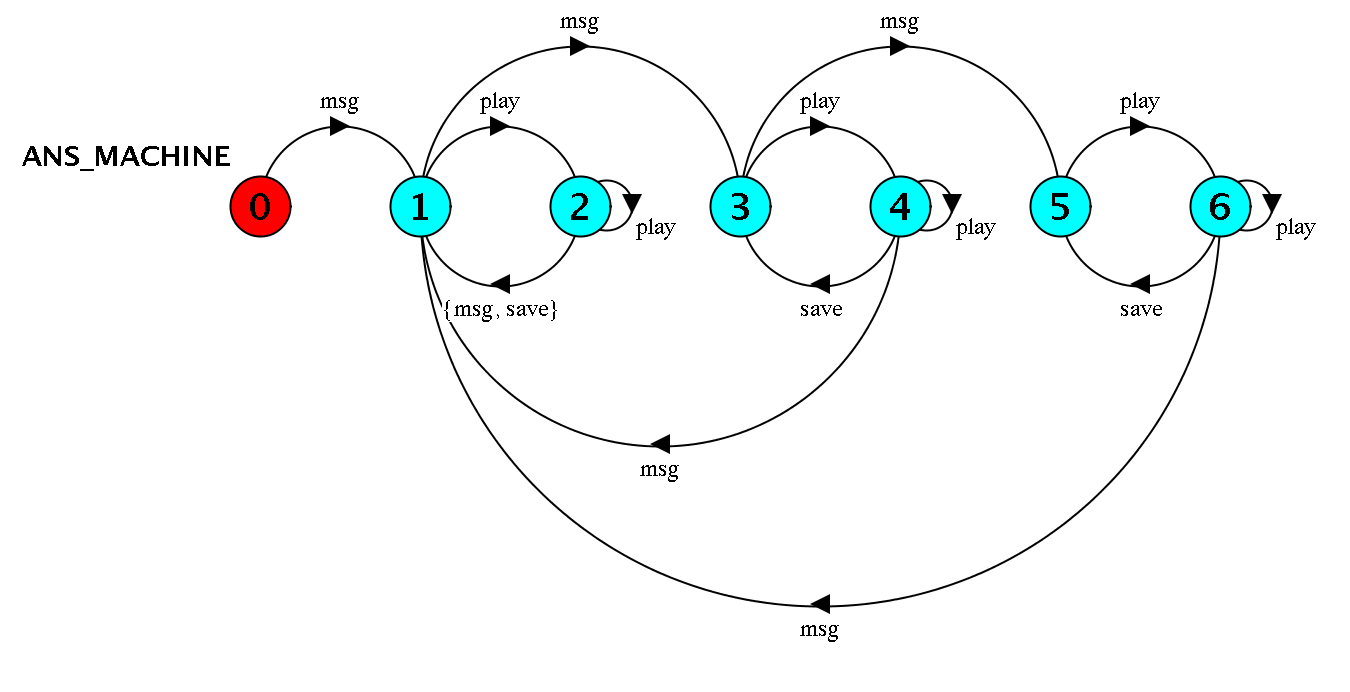
\includegraphics[width=4in]{ans_machine.png}

\begin{verbatim}
ANS_MACHINE = NONE,

NONE = (msg -> ONE),

ONE = (msg -> TWO
      |play -> TEMP1
      ),

TWO = (msg -> THREE
      |play -> TEMP2
      ),

THREE = (play -> TEMP3),

TEMP1 = (play -> TEMP1
        |save -> ONE
        |msg  -> ONE
        ),

TEMP2 = (play -> TEMP2
        |save -> TWO
        |msg  -> ONE
        ),

TEMP3 = (play -> TEMP3
        |save -> THREE
        |msg  -> ONE
        ).
\end{verbatim}


%
%\item Consider the Diverging Counter example of Chapter 10 of GWC09. Prove that $x+y=0$ is an invariant of the $DivergingCounter$ state machine.
%
%(\textsc{Note:} In your proof use style C (in Section 10.1.1) of reasoning about invariants and a similar degree of formalism as in the lecture on this topic.)
%

 \item Consider the FSP specification of a simplified version of the Infusion Pump attached at the end of this assignment.
 Answer the following questions:
    \begin{enumerate}[a.]
    \item Give an example of an action-based trace that causes the infusion pump to terminate without an alarm being raised. \\
      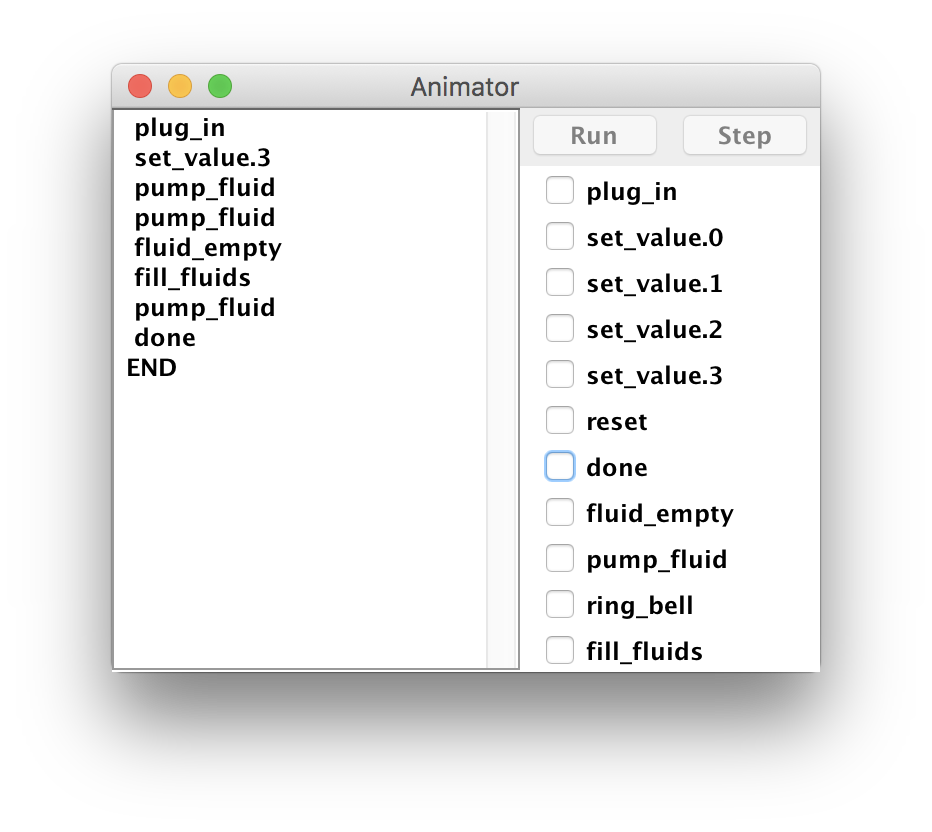
\includegraphics[width=2in]{no_alarm.png} \\
      $trace\_alarm\_not\_raised == \langle plug\_in, set\_value\_3, pump\_fluid, pump\_fluid, fluid\_empty, fill\_fluid, pump\_fluid, done  \rangle $ \\
    \item Give an example of an action-based trace that causes the infusion pump to terminate with an alarm being raised. \\
      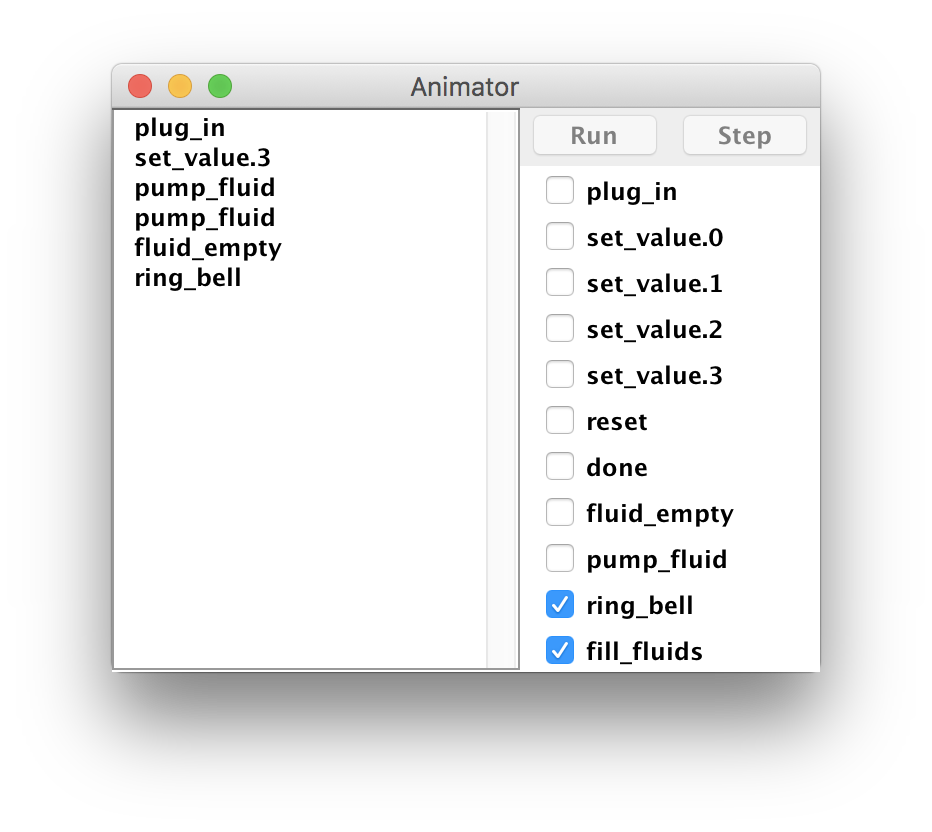
\includegraphics[width=2in]{alarm.png} \\
      $trace\_alarm\_raised ==  \langle plug\_in, set\_value\_3, pump\_fluid, pump\_fluid, fluid\_empty, ring\_bell  \rangle $ \\
    \item Is there a limit to how much medication can be administered to a patient? Explain why or why not. \\
      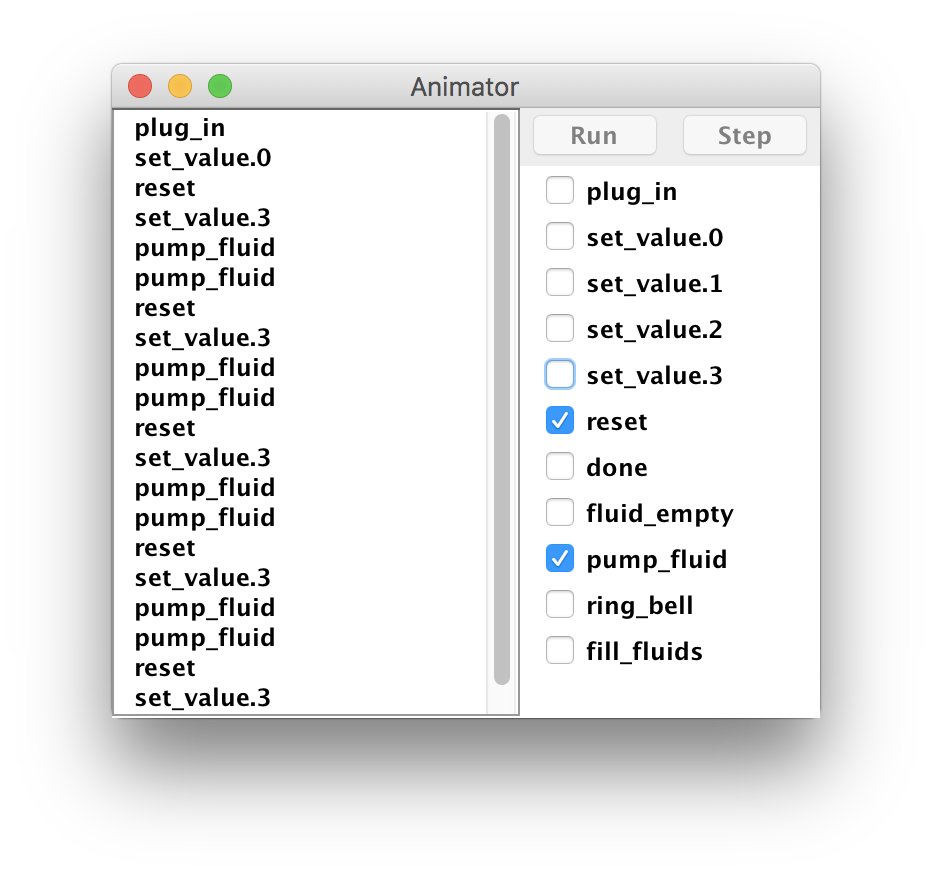
\includegraphics[width=2in]{reset.png} \\
      As it can be seen in the picture, if we reset the machine between filling procedures, it is possible to administer an arbitrary ammount of medicine. This will require human intervention to reset and refill process. \\
      \\
    On it's own the machine has a capacity of $FillAmt=2$. \\  
  \item What happens if the nurse forgets to put any medicine in the bag (i.e., uses a refill amount of 0)? \\
    $ nurse\_forgot == \langle plug\_in, set\_value\_0 \rangle$ \\
    If the nurse makes the machine execute the previous trace, the only options available are to $end$ or $reset$ the machine. The nurse would be able to select another medicine if she/he selects $reset$.
  \item Is it possible for an alarm to sound even if the patient has received the correct and full amount of medicine? \\
    I was unable to find a trace that will end in $ring\_bell$ given the listed conditions. \\ 
    \end{enumerate}

 \item Modify the FSP specification above to add two of the following capabilities, making sure
 to explain in your comments which capabilities you are adding.
 \begin{enumerate}[a.]
    \item self-check at start-up
    \item confirmation of settings
    \item a start and end of treatment time
    \item other error condition detection
    \item ability to set the amount of medicine to be dispensed at each dispensing step
    \item power outage and automatic switch to backup power supply
    \end{enumerate}
 Submit an electronic copy of the modified FSP specification.
\end{enumerate}

\clearpage

\begin{verbatim}
//---------------------------------------------------
//  Infusion Pump modified by Dario
//---------------------------------------------------
//
// Set of actions that can be selected interactively to
// the animation of this model with the LTSA tool.
//
menu AnimationControlMenu = {
    plug_in, set_value[0..3], reset, fill_fluids
}
//---------------------------------------------------
//======================
// Constants and Ranges
//======================
const Max = 3 range Amt = 0 .. Max    
const FillAmt = 2    // Amount in bag initially and after refilling
// Added by Dario:
// Ammout of medicine allowed to be dispensed at each step
//
range Step = 1 .. FillAmt

// Added by Dario:
const SimulationStartTime = 0  // Time when the program was executed.
const EndOfTime = 100 // This is the end of time for the simulation.
range Timestamp = SimulationStartTime .. EndOfTime

//=====================
// Process Definitions
//=====================
//
// Pump starts in power off state
//
PUMP = POWER_OFF,
//
// User must plug pump in before anything else can happen
//
POWER_OFF = (
    plug_in -> SELF_TEST
),

// Added by Dario:
// After plugging the machine, it performs a self-test or fire-up process.
// If successful, proceeds to the SETUP starge, else, it returns the error and ENDS.
// SELF_TEST assumes that failure occurs randomly for educational purposes.
//

SELF_TEST = (
    self_test -> SETUP
    | self_test -> SHOW_ERROR
),

SHOW_ERROR = (show_error -> ERROR), 
//
// Before pump operation starts, user must enter amount of medicine to deliver
// to patient
//
SETUP = (
    set_value[deliver:Amt][step:Step] -> SETUP_CONFIRMATION[deliver][step]
),

//
// Added by Dario: 
// The SETUP_CONFIRMATION step allows the nurse to confirm its selection and proceeed
// to the medicament PUMP process or to go back to SETUP and select another amount of
// medicine.
//

SETUP_CONFIRMATION[deliver:Amt][step:Step] = (
   user_confirmed_settings -> PUMP[deliver][FillAmt][step]
   |user_rejected_settings -> SETUP
),

// 
// Modified by Dario to supply the ammount of medicine defined in step.
// Main operation of pump:
//  User may reset pump at any time
//  When the pump has delivered the amount of medicine requested it goes
//      to the DONE state
//  When fluid runs out, the pump goes into an alarm state
//  Otherwise, the pump delivers one unit of medicine
//

PUMP[deliver:Amt][remaining:Amt][step:Step] = (
    reset -> SETUP
    |
    when (deliver == 0)
        done -> DONE 
    |
    when (remaining < step)
        fluid_empty -> EMPTY_ALARM[deliver][step]
    |
    when (deliver >= step && remaining >= step)
        pump_fluid -> PUMP[deliver-step][remaining-step][step]
    |
    when (deliver < step && remaining >= step)
        pump_fluid -> PUMP[0][remaining - step][step]
),
//
// Error state associated with empty pump:
//  Repeatedly rings bell until user refills the pump
//
EMPTY_ALARM[deliver:Amt][step:Step] = (
    ring_bell -> EMPTY_ALARM[deliver][step]
    | fill_fluids -> PUMP[deliver][FillAmt][step]
),

DONE = END.

//
// Added by Dario:
// POWER_MANAGEMENT is used to control whether the system operates using the energy grid or the backup battery.

POWER_MANAGEMENT = GRID,

GRID = ( tick -> GRID
        | tick -> BACKUP_BATTERY
),

//
// Once the system switches to the backup battery, it remains using it until the machine is stopped.
//
BACKUP_BATTERY = (tick -> BACKUP_BATTERY).

//
// Clock used to store the simulation time, on each tick it gets increased by one until it reaches the end of time.
CLOCK = TICK[SimulationStartTime],

TICK[t:Timestamp] = (
    when(t < EndOfTime)
        tick -> TICK[t + 1]
    |
    when(t >= EndOfTime)
        tick -> ERROR
).
//
// Run Clock, Power Management and the Pump in parallel.
//
|| CLOCK_PUMP = (CLOCK || PUMP || POWER_MANAGEMENT).

\end{verbatim}
\end{document}

\end{enumerate}

\end{document}
